\section{Felhasználói követelmények}
	\paragraph{}
	A Sapi3D alkalmazás web alapú, ezért mindenki számára elérhető
	a fő célja, hogy egy 3D modellként jelenítse meg a Sapientia EMTE Marosvásárhely-i karának a fő épületét, illetve ennek fontosabb helyeit, mint pl. tanszékek, titkárság stb.
	A rendszer fontosabb funkcionalitásait és az ezeket igénybe vevő szerepköröket a \ref{fig:UseCase} ábra szemlélteti.
	\paragraph{}
	A rendszer működése érdekében semmi előfeltételt nem kell teljesítenie a felhasználónak mivel a weboldal egyik része teljesen nyitott, elérhető bárki számára. A rendszer megértésének érdekében tekintsük meg a \ref{fig:UseCase} ábrát amely bemutatja a rendszer különböző részeit.
	\paragraph{}
	Az \ref{fig:UseCase} ábrát tekintve észre vehetünk három aktort amelyek különböző vagy ugyan azt a tevékenységet végezhetik el. Megfigyelhető, hogy a visitor(látogató) átváltozhat user felhasználóvá. Az admin felhasználó tulajdonképpen egy user felhasználó aki admin jogosultsággal rendelkezik. A user és admin típusú felhasználók azok a személyek akik az oldal karbantartásáért felelősek.
	\paragraph{}
	Bármely felhasználó, aki egy böngészőből megnyitja az oldalt, a látogató kategóriából került.Ez a fajta felhasználó megtekintheti a 3d modellt, körbe sétálhatja és el tud jutni pl.titkárságra. Amint megnyílt az oldal rögtön látható az egyetemről készített modell. Ezen a modellen tud nézelődni, esetleg körbe is tudja járni, vagy adott helységekre el is tud jutni(például: titkárság, adott tanszék). Ezen kívül lehetősége van információk, elérhetőségek, események részleteinek elolvasására is. Minden visitor(látogató) ugyan akkor leírhatja saját véleményét, meglátásait az oldallal kapcsolatban is. A fent említett műveletek elvégzéséhez nem kell sem bejelentkezés, sem regisztráció.
	\paragraph{}
	Amint már említettem a visitor(látogató) át tud alakulni user felhasználóra. Ez abban különbözik a látogatótól, hogy be is tud jelentkezni és több műveletet tud elvégezni. A műveletek elvégzésének engedélyezése azon múlik hogy a bejelentkező felhasználó user vagy admin. Ha user képes bejelentkezni, eseményeket megadni, az egyetemmel kapcsolatos információkat módosítani, új 3D modellt is hozzáadni. Ezeken kívül mivel jelen van bejelentkezés így a kijelentkezés opció is a rendelkezésükre áll.
	\paragraph{}
	A regisztrációs feladatot egy admin jogosultsággal rendelkező ember végezheti el. Nem csak a regisztrálás tartozik az ő feladatköreihez hanem a userek törlése is az ő feladata. Ezen plusz műveletek mellett szintén elvégezheti az user és a visitor műveleteit is.
	\begin{figure}
		\centering
		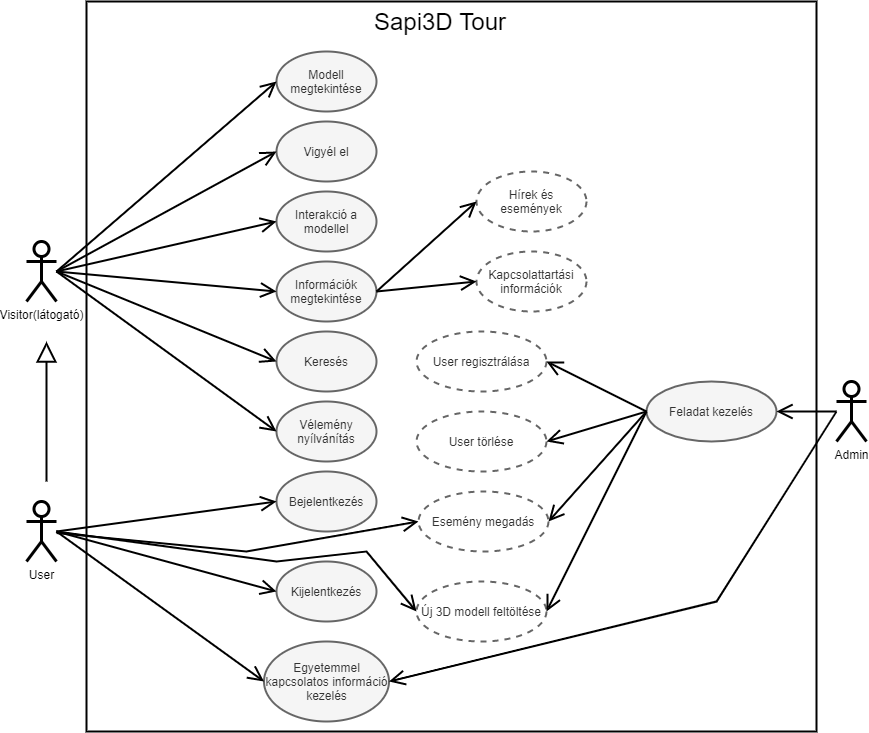
\includegraphics[scale=0.6]{figures/images/UseCase.png}
		\caption{Use Case diagram}
		\label{fig:UseCase}
	\end{figure}
\pagebreak